\documentclass[25pt, a0paper, portrait]{tikzposter}

\usepackage{graphicx}
\usepackage{wrapfig}
\usepackage{ETbb}
\usepackage[fontsize=28pt]{fontsize}
% \usepackage{microtype}  % conflicts with hyperref and tikzposter, see https://tex.stackexchange.com/questions/481636/incompatibility-between-tikzposter-class-microtype-and-hyperref-package
\usepackage{hyperref}
\usepackage{qrcode}

% \title{The Journal of Open Source Software}
% \author{\emph{EditorsWarrick Ball}
% \date{\today}
% \institute{University of Birmingham}
% \usetheme{Simple} % Default, Rays, Basic, Simple, Envelope, Wave, Board, Autumn, and Desert
% \usecolorstyle{Denmark}
% \titlegraphic{logo_large.png}
\settitle{}

% https://tex.stackexchange.com/questions/254257/tikzposter-and-doi-package-conflict
\def\HyperFirstAtBeginDocument#1{#1}
\begin{document}

% Title block with title, author, logo, etc.
% \maketitle

\makeatletter
    \setlength{\TP@blocktop}{.485\textheight}
\makeatother

% https://github.com/openjournals/joss/blob/main/public/logo_large.jpg
% logo, QR code

\block{}{
  \begin{center}
    
\includegraphics[width=0.5\textwidth]{joss-logo-transparent-crop.png} \\
    \textbf{Editorial board} \\
   \small Patrick Diehl, Daniel S.~Katz, Luiz Irber, Mark A.~Jensen, Stefan Appelhoff, Yasmin Mzayek, Frederick Boehm, Øystein Sørensen, Kanishka B.~Narayan, Kristen Thyng, Eloisa Bentivegna, Ana Trisovic, Charlotte Soneson, Jacob Schreiber, Sehrish Kanwal, Hugo Ledoux, Vissarion Fisikopoulos, Britta Westner, Jeff Gostick, Jayaram Hariharan, Dana Solav, Marcos Vital, Christopher R.~Madan, Dan Foreman-Mackey, Johanna Bayer, Juanjo Bazán, Fabian Scheipl, Kyle Niemeyer, Fabian-Robert Stöter, Michael Mahoney, Bonan Zhu, Nikoleta Glynatsi, Kevin M.~Moerman, Hauke Schulz, Andrew Stewart, Mojtaba Barzegari, Chris Vernon, Adam R.~Jensen, Jarvist Moore Frost, Kelly Rowland, Vincent Knight, Martin Fleischmann, Josh Borrow, Hugo Gruson, Prashant K Jha, Mehmet Hakan Satman, Marcel Stimberg, Axel Donath, Samuel Forbes, Renata Diaz, Olivia Guest, Sarath Menon, Taher Chegini, Fei Tao, Ivelina Momcheva, Warrick Ball, Antonia Mey, Jed Brown, Andrew Quinn, George K.~Thiruvathukal, Susan Holmes, Matthew Feickert, Olexandr Konovalov, Philip Cardiff, Aoife Hughes, Monica Bobra, Paul La Plante, Gabriela Alessio Robles, Lucy Whalley, Lorena Pantano, Jonny Saunders, Claudia Solis-Lemus, Brian McFee, Arfon Smith, Oskar Laverny, Rachel Kurchin, Richard Gowers, Sebastian Benthall, Elizabeth DuPre, Rocco Meli, Rohit Goswami, Julia Romanowska, Rachel Wegener, Anjali Sandip, Pierre de Buyl, Teon Brooks, Adam Tyson, Gracielle Higino, Sébastien Boisgérault, Mengqi Zhao, Tristan Miller, AHM Mahfuzur Rahman, Sophie Beck, Frauke Wiese, Adi Singh, Beatriz Costa Gomes
  \end{center}
}

\begin{columns}
\column{0.5} \block{About}{The Journal of Open Source Software (JOSS)
  is an academic journal (ISSN 2475-9066) that publishes short
  articles describing open source software with a research
  application.  The review process includes checking that the
  software itself
  \href{https://joss.readthedocs.io/en/latest/review_checklist.html}{meets
    some modern standards}, including having documentation, tests
  (preferably automated), and community guidelines.  This way, JOSS
  aims to give software creators a citable artefact
  through which their research contribution can be recognised,
  and to encourage them to use good software practice.}

\block{Publication statistics}{
  \begin{center}
    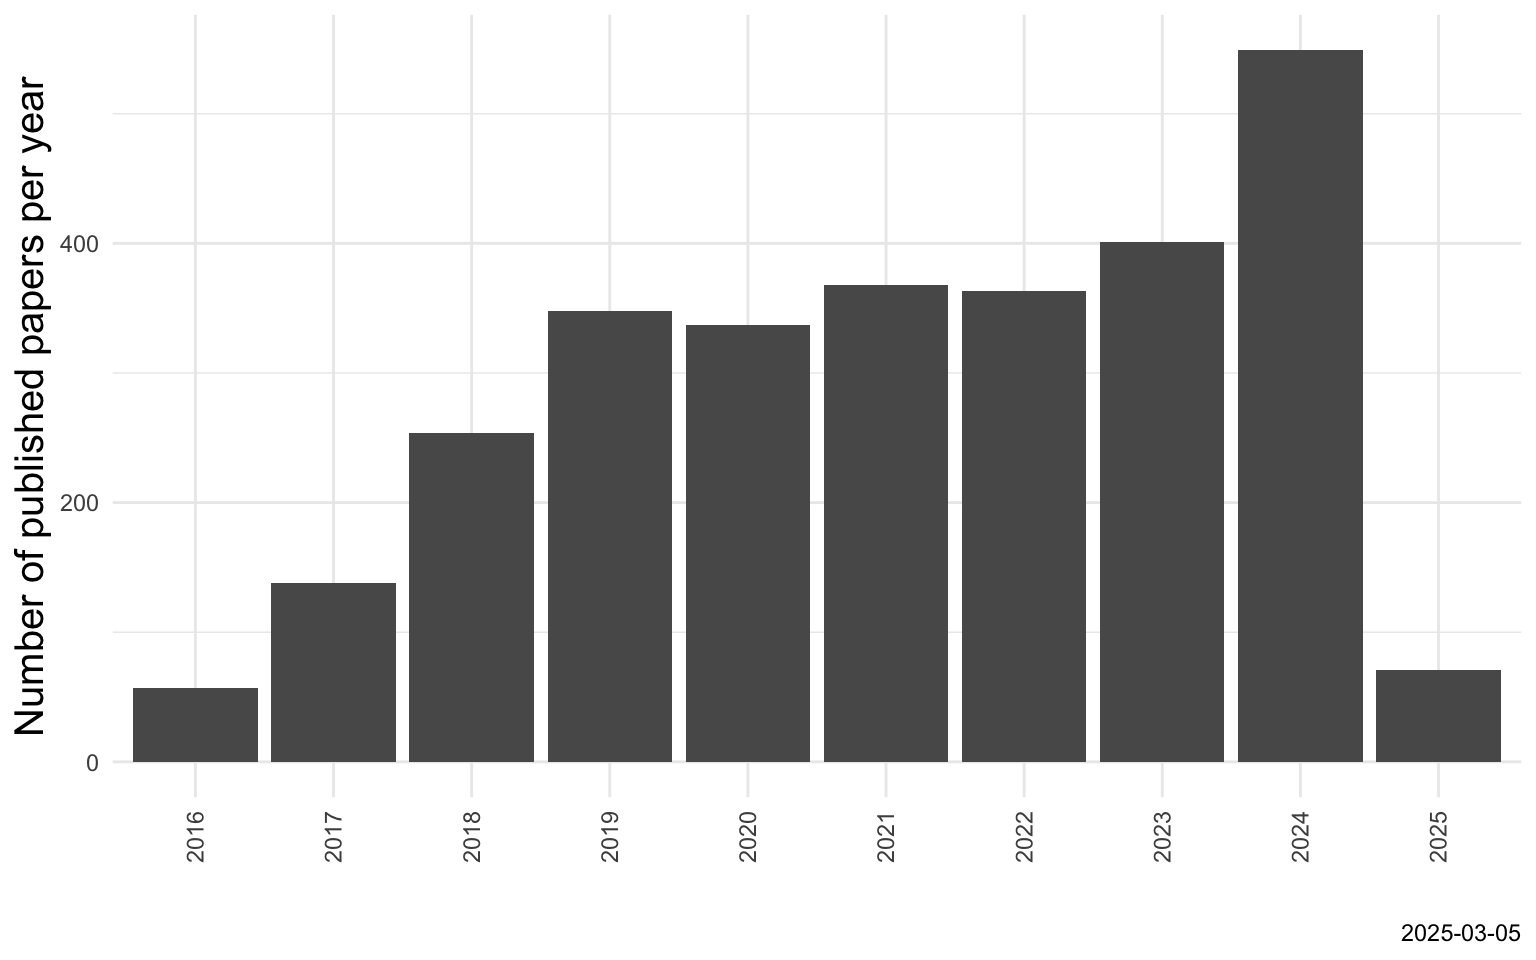
\includegraphics[width=0.43\textwidth]{joss-papers-per-year.png}
  \end{center}
  \begin{center}
    \emph{Most-cited articles}:
  \begin{tabular}{p{0.62\linewidth}@{\quad}cc}
    \textbf{Title} & \textbf{Date} & \textbf{Citations} \\
    \href{https://dx.doi.org/10.21105/joss.01686}{Welcome to the Tidyverse} & 2019-11-21 & 9\,431 \\
    \href{https://dx.doi.org/10.21105/joss.00861}{UMAP: Uniform Manifold Approximation and Projection}
    & 2018-09-02 & 4\,858 \\
    \href{https://dx.doi.org/10.21105/joss.03021}{seaborn: statistical data visualization} & 2021-04-06 & 2\,652 \\
    \href{https://dx.doi.org/10.21105/joss.03139}{performance: An R Package for Assessment, Comparison and Testing of Statistical Models} & 2021-04-21 & 1\,574 \\
    \href{https://dx.doi.org/10.21105/joss.00024}{corner.py: Scatterplot matrices in Python} & 2016-06-08 & 1\,313 \\
  \end{tabular}
  \end{center}
}

\block{Get involved}{
 \href{https://joss.readthedocs.io/en/latest/submitting.html}{\textbf{Publish your code!}}
  JOSS is developer-friendly.  If you've already developed a significant research code
  with an open source licence, good documentation and automatic tests,
  we think it should only take an hour or two to prepare and submit your paper to JOSS.
  \begin{center}
  \qrcode{https://joss.theoj.org/}
  \end{center}
  \href{https://reviewers.joss.theoj.org/join}{\textbf{Volunteer to review!}}
  The review process is used as an opportunity to help creators improve their software.
  Reviewers are encourage to open issues and iteratively improve the software, rather
than providing a few monolithic reviews, several weeks apart.}

\column{0.5}
\block{Publication workflow}{
  \begin{center}
    \includegraphics[width=0.42\textwidth]{JOSS-flowchart-updated.pdf}
  \end{center}
}

\block{Behind the scenes}
{JOSS streamlines its editorial processes by using software
  development tools.  Pre-review and review discussions happen in
  GitHub issues.  Many editorial steps are handled by the editorial
  bot: a \href{https://buffy.readthedocs.io/}{Ruby package}
  that interacts with GitHub via its API to do things
  like generate the pre-review and review issues, post checklists,
  recompile the article PDF on request, check reference DOIs, and more! \\
  \\
  Manuscripts are prepared in a flavour of Markdown and compiled to
  PDF via Pandoc.  JOSS's compilation process is available to authors
  as a GitHub action, so compliance can be checked automatically.
}

% \begin{subcolumns}
%   \subcolumn{0.45}
%   \block{JOSS homepage}{\begin{center}
%       \url{https://joss.theoj.org} \\
%       
\includegraphics[width=0.15\textwidth]{joss-qr.png}
%   \end{center}}
%   \subcolumn{0.55}
  \block{About this poster}{
Presented by Patrick Diehl and Daniel S. Katz at the \emph{2nd Annual Conference of the US Research Software Engineering Association} in Albuquerque, NM, 15--17 Oct 2024. Publication workflow diagram by Kyle Niemeyer. \\

\begin{wrapfigure}[5]{r}{10cm}\vskip-1em\includegraphics[width=\linewidth]{by.png}\end{wrapfigure}
Licensed under a Creative Commons Attribution 4.0 \\
International License: \\
\url{https://creativecommons.org/licenses/by/4.0/}
}
% \end{subcolumns}


\end{columns}

\end{document}
